
\documentclass{beamer}
%
% Choose how your presentation looks.
%
% For more themes, color themes and font themes, see:
% http://deic.uab.es/~iblanes/beamer_gallery/index_by_theme.html
%
\mode<presentation>
{
  \usetheme{default}      % or try Darmstadt, Madrid, Warsaw, ...
  \usecolortheme{default} % or try albatross, beaver, crane, ...
  \usefonttheme{default}  % or try serif, structurebold, ...
  \setbeamertemplate{navigation symbols}{}
  \setbeamertemplate{caption}[numbered]

} 

\setbeamertemplate{footline}[text line]{%
  \parbox{\linewidth}{\vspace*{0pt}
    \begin{flushright}Copyright \textcopyright\ 2016 \insertshortauthor.\end{flushright}}}

\usepackage[english]{babel}
\usepackage[utf8x]{inputenc}
\usepackage{color}

\usepackage{tikz}
\usetikzlibrary{mindmap,trees}

\linespread{1.3}
\definecolor{links}{HTML}{2A1B81}
\hypersetup{colorlinks,linkcolor=,urlcolor=links}

\title[Your Short Title]{Operations research with Julia and JuMP }
\author{Pedro Belin Castellucci}
\date{November, 2016}


\begin{document}

\setbeamercolor{title}{fg=black}
\setbeamercolor{frametitle}{fg=black}


\begin{frame}
  \titlepage
\end{frame}


\section{Introduction}

\begin{frame}{Mathematical programming}

  \begin{figure}[htpb]
    \centering
  \scalebox{0.7}{
    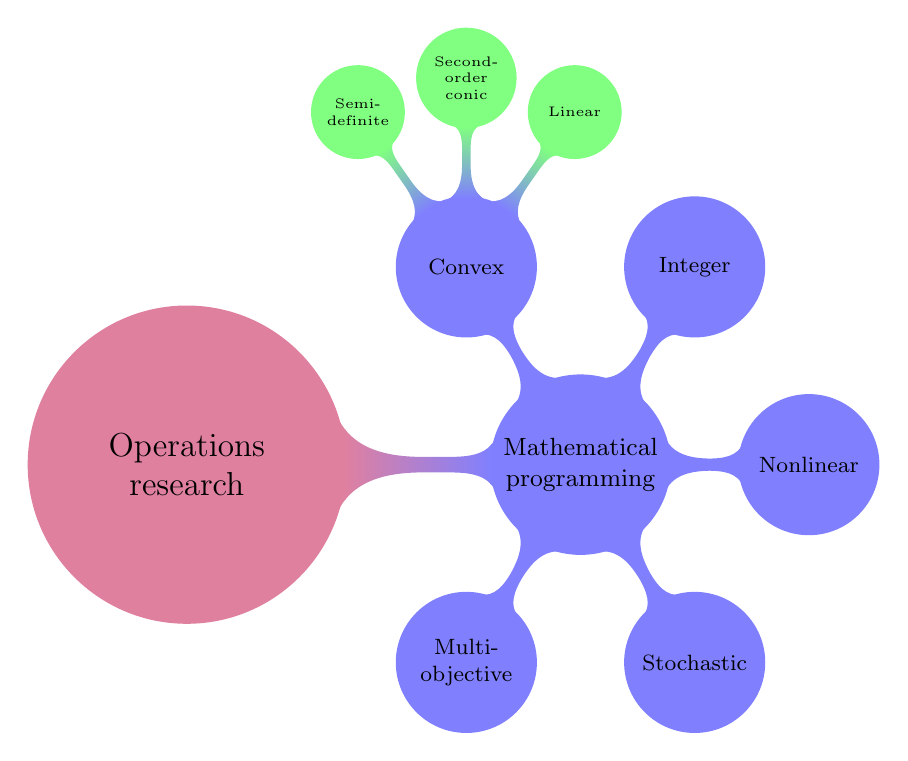
\begin{tikzpicture}

%      \pgflowlevel{\pgftransformscale{0.7}}
      
      \path[mindmap, concept color=purple!50, text=black]
      node[concept] {Operations \\research}
      [clockwise from=0]
      child[concept color=blue!50] {
        node[concept] {Mathematical programming}
        [clockwise from=120]
        child { node[concept] {Convex}
          child [concept color=green!50, grow=125]{ node[concept] {Semi-definite} } 
          child [concept color=green!50, grow=90] {node[concept] {Second-order conic}}
          child [concept color=green!50, grow=55] {node[concept] {Linear}}
        }
        child { node[concept] {Integer} }
        child { node[concept] {Nonlinear} }
        child { node[concept] {Stochastic} }
        child { node[concept] {Multi-objective} }
      };
    \end{tikzpicture}
  }
  \caption{Information from \url{https://en.wikipedia.org/wiki/Mathematical_optimization}.}
  \end{figure}

\end{frame}


\begin{frame}{Which can JuMP handle?}

  \begin{figure}[htpb]
    \centering
  \scalebox{0.7}{
    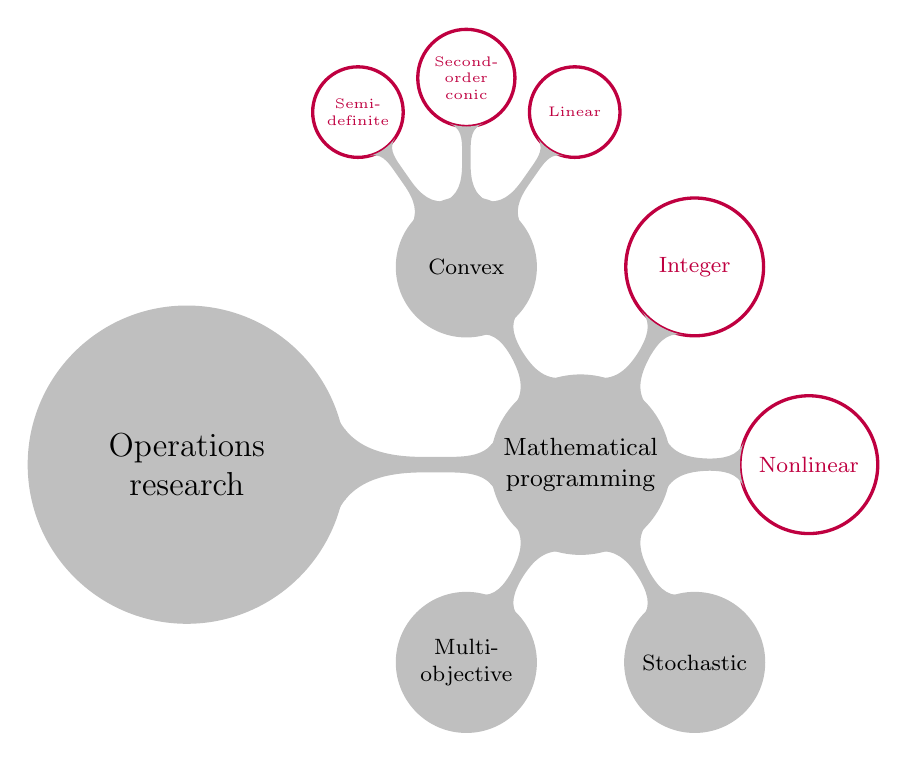
\begin{tikzpicture}

%      \pgflowlevel{\pgftransformscale{0.7}}
      
      \path[mindmap, concept color=gray!50, text=black]
      node[concept] {Operations \\research}
      [clockwise from=0]
      child[concept color=gray!50] {
        node[concept] {Mathematical programming}
        [clockwise from=120]
        child { node[concept] {Convex}
          child [concept color=gray!50, grow=125]{ node[draw, circle, purple] {Semi-definite} } 
          child [concept color=gray!50, grow=90] { node[draw, circle, purple] {Second-order conic}}
          child [concept color=gray!50, grow=55] { node[draw, circle, purple] {Linear}}
        }
        child { node[draw, circle, purple] {Integer} }
        child { node[draw, circle, purple] {Nonlinear} }
        child { node[concept] {Stochastic} }
        child { node[concept] {Multi-objective} }
      };
    \end{tikzpicture}
  }
  \caption{For JuMP documentation go to \url{http://www.juliaopt.org/JuMP.jl/0.15/}.}
  \end{figure}

\end{frame}


\begin{frame}{What will we do?}

  \begin{figure}[htpb]
    \centering
  \scalebox{0.7}{
    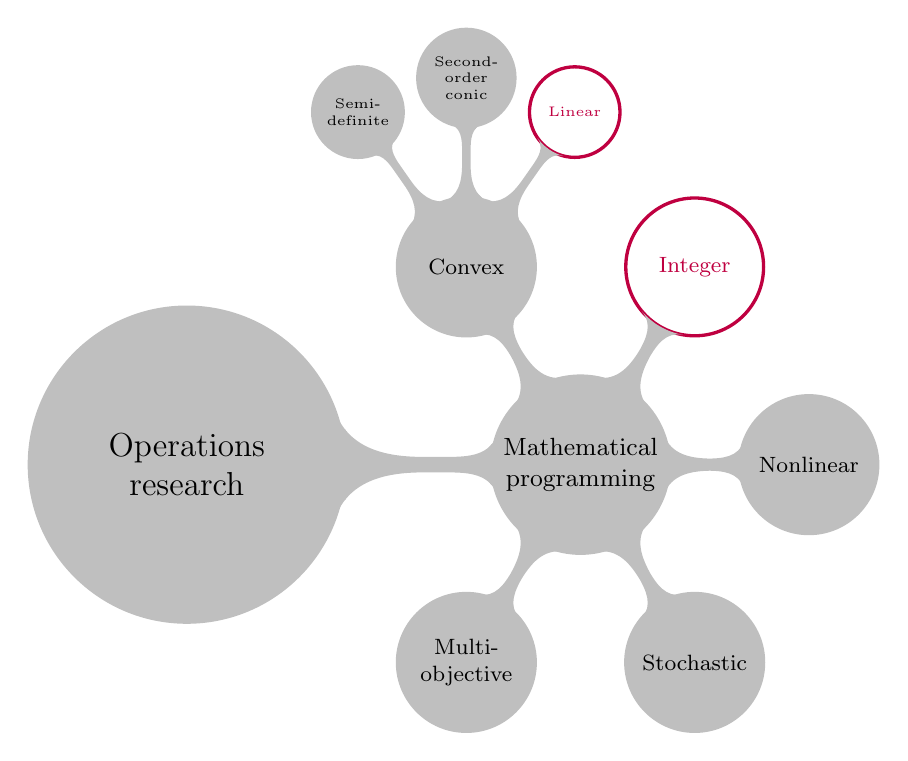
\begin{tikzpicture}

%      \pgflowlevel{\pgftransformscale{0.7}}
      
      \path[mindmap, concept color=gray!50, text=black]
      node[concept] {Operations \\research}
      [clockwise from=0]
      child[concept color=gray!50] {
        node[concept] {Mathematical programming}
        [clockwise from=120]
        child { node[concept] {Convex}
          child [concept color=gray!50, grow=125]{ node[concept] {Semi-definite} } 
          child [concept color=gray!50, grow=90] { node[concept] {Second-order conic}}
          child [concept color=gray!50, grow=55] { node[draw, circle, purple] {Linear}}
        }
        child { node[draw, circle, purple] {Integer} }
        child { node[concept] {Nonlinear} }
        child { node[concept] {Stochastic} }
        child { node[concept] {Multi-objective} }
      };
    \end{tikzpicture}
  }
  \caption{For JuMP documentation go to \url{http://www.juliaopt.org/JuMP.jl/0.15/}.}
  \end{figure}

\end{frame}

\begin{frame}
  \frametitle{What is mixed linear integer optimization?}
  \pause

  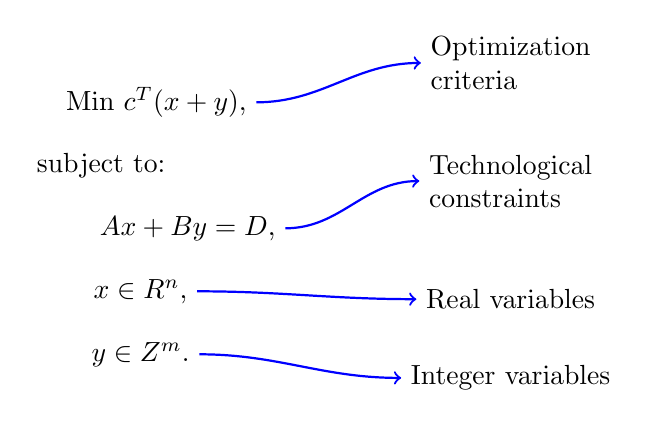
\begin{tikzpicture}
    \node (obj) at (-0.5, 0) {Min $c^T (x + y)$,};
    \node (st) at (-1.2,-0.8) {subject to:};
    \node (const1) at (-0.1,-1.6) {$Ax + By = D$,};
    \node (const2) at (-0.7,-2.4) {$x \in \mathbb{R}^n$,};
    \node (const3) at (-0.7,-3.2) {$y \in \mathbb{Z}^m$.};
    \pause
    
    \node [align=left] (objLabel) at (4,0.5) {Optimization\\criteria};
    \draw [blue, thick, ->] (obj) to[out=0, in=180] (objLabel); 
    \pause
    
    \node [align=left] (const1Label) at (4,-1) {Technological\\ constraints};
    \draw [blue, thick, ->] (const1) to[out=0, in=180] (const1Label); 
    \pause
    
    \node [align=left] (const2Label) at (4, -2.5) {Real variables};
    \draw[blue, thick, ->] (const2) to[out=0, in=180] (const2Label);
    \pause
    
    \node [align=left] (const3Label) at (4, -3.5) {Integer variables};
    \draw[blue, thick, ->] (const3) to[out=0, in=180] (const3Label);
  \end{tikzpicture}
  
\end{frame}

\begin{frame}
  \frametitle{An example}
    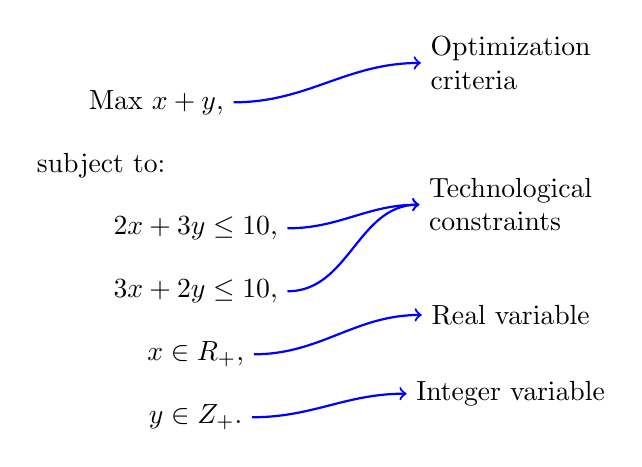
\begin{tikzpicture}
    \node (obj) at (-0.5, 0) {Max $x + y$,};
    \node (st) at (-1.2,-0.8) {subject to:};
    
    \node (const1) at (0,-1.6) {$2x + 3y \leq 10$,};
    \node (const2) at (0,-2.4) {$3x + 2y \leq 10$,};
    
    \node (const3) at (0, -3.2) {$x \in \mathbb{R}_+$,};
    \node (const4) at (0, -4.0) {$y \in \mathbb{Z}_+$.};

    \pause
    \node [align=left] (objLabel) at (4,0.5) {Optimization\\criteria};
    \draw [blue, thick, ->] (obj) to[out=0, in=180] (objLabel); 
    
    \node [align=left] (const1Label) at (4,-1.3) {Technological\\ constraints};
    \draw [blue, thick, ->] (const1) to[out=0, in=180] (const1Label);
    \draw [blue, thick, ->] (const2) to[out=0, in=180] (const1Label); 
    
    \node [align=left] (const3Label) at (4, -2.7) {Real variable};
    \draw[blue, thick, ->] (const3) to[out=0, in=180] (const3Label);
    
    \node [align=left] (const4Label) at (4, -3.7) {Integer variable};
    \draw[blue, thick, ->] (const4) to[out=0, in=180] (const4Label);
  \end{tikzpicture}
\end{frame}


\begin{frame}
  \frametitle{JuMP - Julia for Mathematical Optimization}

  \footnotesize
  \begin{itemize}
    \item <2-> [] Domain-specific modeling language.
    \item <3-> [] User friendliness.
    \item <4-> [] Speed:
      \begin{itemize}
        \item [] Creates problems at similar speed of other modeling languages (e. g. AMPL).
        \item [] Communicates with solver in memory.
      \end{itemize}
    \item <5-> [] Solver independence:
      \begin{itemize}
      \item [] Current supports Artelys Knitro, Bonmin, Cbc, Clp, Couenne, CPLEX, ECOS, FICO Xpress, GLPK, Gurobi, Ipopt, MOSEK, NLopt, and SCS.
      \end{itemize}
  \end{itemize}
  
\end{frame}


\begin{frame}
  \centering
  \vfill
%  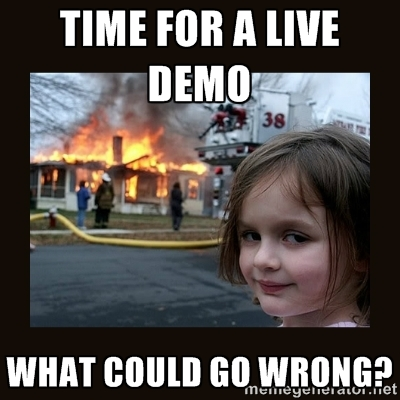
\includegraphics[scale=0.6]{live-demo.jpg}
  \vfill
\end{frame}


\begin{frame}
  \frametitle{Exercise - The knapsack problem}
  {\footnotesize Let $i \in I$ be an item with value $v_i$ and weight $c_i$. We want to choose the most valuable subset of items to carry in a knaspack without violating its capacity $C$. Let $x_i \in \{0, 1\}$, $i \in I$, indicate whether item $i$ is put into the knapsack. The following integer program solves our knapsack problem.}

  \vspace{-1cm}
  \begin{center}
  \begin{equation*}
  Max\ \sum_{i \in I} v_i x_i: \sum_{i \in I} c_i x_i \leq C, \ x_i \in \{0, 1\}, i \in I.
  \end{equation*}
  \end{center}

  \footnotesize
  \begin{enumerate}
  \item Solve the instance on the file example.dat.
  \item As output, provide how many and which items were taken and their aggregated value.
  \end{enumerate}
  
\end{frame}


\begin{frame}
  \frametitle{Exercise - Scheduling TV commercials}
  You are in charge of a scheduling commercials during a TV show. By contract, you must run all the commercials $c \in C$ during the show. Each commercial $c$ has the duration $t_c \leq 3$, $c \in C$, in minutes. The show may have any number of intervals, however, you know that there might be an audience drop for every interval. Also, to prevent audience loss, intervals must not be greater than 3 minutes. 
\end{frame}


\begin{frame}
  \frametitle{Exercise - Scheduling TV commercials}

  \footnotesize

  Let $x_{ic} \in \{0, 1\}$ indicate whether commercial $c$ is schedule to interval $i$. The following integer program solves the problem.
  
  \begin{equation*}
  Min\ \sum_{i=1}^{|C|} y_i,
  \end{equation*}

  subject to:

  \vspace{-0.7cm}
  \begin{alignat*}{2}
    &\sum_{c \in C} t_c x_{ic} \leq 3 y_i && \quad i \in \{1, \ldots, |C|\},\\
    & \sum_{i=1}^{|C|} x_{ic} = 1, && \quad c \in C,\\
    & y_i \in \{0, 1\}, && \quad i \in \{1, \ldots, |C|\},\\
    & x_{ic} \in \{0, 1\}, && \quad i \in \{1, \ldots, |C|\}, c \in C. 
  \end{alignat*}

Implement the model and solve it using random input data.
  
\end{frame}


\begin{frame}
  \frametitle{One step further -- callbacks}

  \begin{enumerate}
  \item [] Lazy constraints
  \item [] User cuts
  \item [] User heuristics
  \item [] Solver progress
  \item [] Informational
  \end{enumerate}

    \vfill \footnotesize
  More info at: \url{https://jump.readthedocs.io/en/latest/callbacks.html}
\end{frame}


\begin{frame}
  \frametitle{Lazy constraints}
  Called when new solutions are found.

  \begin{block}{Code:}\footnotesize
    
    \textcolor{violet}{\textbf{function}} myLazyConstraint(cb)
    
    \hspace{1cm}    ...
    
    \hspace{1cm}    @lazyconstraint(cb, myconstraint, localcut=true)

    \textcolor{violet}{\bf end}
    
    addlazycallback(m, myLazyConstraint)

    solve(m)
  \end{block}

\end{frame}


\begin{frame}
  \frametitle{User cuts}
  Called when solver reaches a new node in the branch-and-bound tree

  \begin{block}{Code:}\footnotesize
    
    \textcolor{violet}{\textbf{function}} myUserCut(cb)
    
    \hspace{1cm}    ...
    
    \hspace{1cm}    @usercut(cb, myconstraint, localcut=true)

    \textcolor{violet}{\bf end}
    
    addcutcallback(m, myUserCut)

    solve(m)
  \end{block}
  
\end{frame}


\begin{frame}
  \frametitle{User heuristics}

  Create solutions and submit them back to the solver

  \begin{block}{Code:}\footnotesize
    
    \textcolor{violet}{\textbf{function}} myHeuristic(cb)
    
    \hspace{1cm}    ...
    
    \hspace{1cm}    setsolutionvalue(cb, x, value)
    
    \hspace{1cm}    addsolution(cb)

    \textcolor{violet}{\bf end}
    
    addheuristiccallback(m, myHeuristic)

    solve(m)
  \end{block}

\end{frame}


\end{document}


%%% Local Variables:
%%% mode: latex
%%% TeX-master: t
%%% End:
